\documentclass{article}
\usepackage[utf8]{inputenc}
\usepackage[
    margin = 3cm
]{geometry}
\usepackage{graphicx}
\usepackage{booktabs}
\usepackage{etoolbox}

\usepackage{gridlayout}

\begin{document}

Some text before the grid layout...

\begin{gridlayout}[\textwidth]
    \begin{row}{4cm}
        \begin{cell}{0.2}
            Foo 1
        \end{cell}
        \begin{cell}{0.4}
            Bar 1
        \end{cell}
        \begin{cell}{0.2}
            Baz 1
        \end{cell}
    \end{row}
    \begin{row}{6cm}
        \begin{cell}{0.1}
            Lorem ipsum dolor sit amet 
        \end{cell}
        \begin{cell}{0.5}
            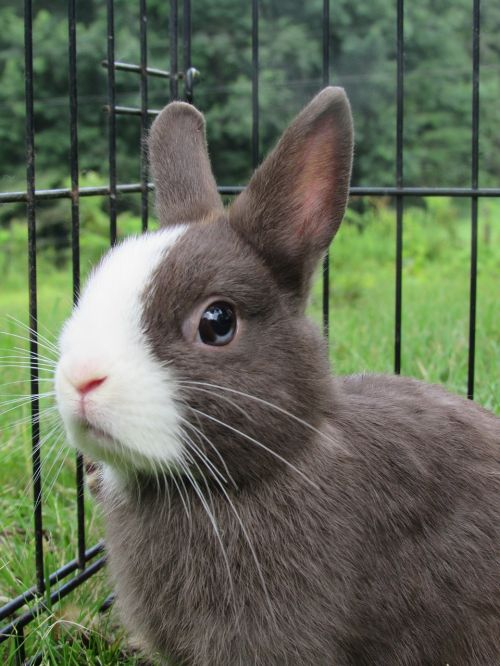
\includegraphics[height = 6cm]{img/rabbit.jpg}
        \end{cell}
        \begin{cell}{0.4}
            \centering
            \begin{tabular}{lll}
                \toprule
                Foo & Bar & Baz \\
                \midrule
                123 & 456 & 789 \\
                abc & def & ghi \\
                \bottomrule
            \end{tabular}
        \end{cell}
    \end{row}
\end{gridlayout}

Some text after the grid layout...

\end{document}